\documentclass[aspectratio=169]{beamer}
\usepackage[UTF8,heading,fontset=none]{ctex} % 中文支持
\usepackage{ncepu-beamer} % 应用主题

\usepackage{color}
\usepackage{amsmath}
\usepackage{tikz}        % 绘图
\usepackage{minted}      % 代码高亮
\usepackage{hyperref}    % 超链接
\usepackage{subcaption}  % 创建子图
\usepackage{algorithm2e} % 伪代码
% 表格
\usepackage{booktabs}
\usepackage{multirow}
\usepackage{diagbox}
\usepackage{makecell}

% --------------- 字体设置 --------------- %
%% 配置方式见 README.md
%% 如果不想使用自定义字体,可以注释掉下面的设置
%% 并且删除 ctex 包的 `fontset=none` 选项
\usepackage{fontspec}
\setmainfont{HarmonyOS Sans}
\setsansfont{HarmonyOS Sans}
\setmonofont{CodeNewRoman Nerd Font}
\setCJKmainfont{HarmonyOS Sans SC}
\setCJKsansfont{HarmonyOS Sans SC}
\setCJKmonofont{HarmonyOS Sans SC}
% --------------- 字体设置 --------------- %

% --------------- svg 设置 --------------- %
\usepackage[notransparent]{svg} % 插入 svg 矢量图
\setsvg{
  %% 设置 inkscape 路径(inkscape 用于处理 svg 矢量图)
  % inkscapeexe={"C:/Program Files/Inkscape/bin/inkscape.com"}, % Windows
  inkscapeexe={"/usr/bin/inkscape"}, % Linux
  %% 设置 svg 文字随图片缩放
  inkscapelatex=false
}
%% NOTE: draw.io 中的文本需要关闭自动换行和格式化文本
% --------------- svg 设置 --------------- %

% 输入信息
\title{Heterogeneity-Aware Proactive Elastic Resource Allocation for Serverless Applications}
\subtitle{基于异构性感知的无服务器应用主动弹性资源分配}
\author{刘肇泽}
\institute{Distributed System Group, NCEPU}
\date{\today}

\begin{document}

\begin{frame}[noframenumbering]

  \titlepage

\end{frame}

\begin{frame}{目录}

  \centering
  \begin{minipage}{0.5\textwidth}
    \tableofcontents
  \end{minipage}

\end{frame}

% 从这里开始你的创作

% -------------------------------------------------------- %
\section{无服务计算背景}
% -------------------------------------------------------- %

\begin{frame}{无服务器计算背景}{概述}
  无服务器计算 (Serverless Computing),也称为函数即服务 (Function as a Service, FaaS),是一种新型云计算模型。用户仅需将函数代码上传至云端,就可以直接发送请求触发函数执行,其底层的运行环境和计算资源由云服务提供商管理。
\end{frame}

\begin{frame}{无服务器计算背景}{云函数部署示例}
  腾讯云云函数 (Serverless Cloud Function, SCF) 部署示例:
  \begin{columns}
    \column{0.5\textwidth}
    \begin{figure}
      \centering
      \includegraphics[width=\textwidth]{img/serverless-background/scf-deploy-1.png}
    \end{figure}

    \column{0.5\textwidth}
    \begin{figure}
      \centering
      \includegraphics[width=\textwidth]{img/serverless-background/scf-deploy-2.png}
    \end{figure}
  \end{columns}
\end{frame}

\begin{frame}{无服务器计算背景}{函数调用示例}
  创建函数 URL:
  \begin{figure}
    \centering
    \includegraphics[height=0.45\textheight]{img/serverless-background/scf-invoke-1.png}
  \end{figure}
  直接通过访问 URL 触发函数执行:
  \begin{figure}
    \centering
    \includegraphics[height=0.15\textheight]{img/serverless-background/scf-invoke-2.png}
  \end{figure}
\end{frame}

\begin{frame}{无服务器计算背景}{大量模板}
  \begin{figure}
    \begin{subfigure}{0.45\textwidth}
      \centering
      \includegraphics[height=0.7\textheight]{img/serverless-background/scf-template-1.png}
      \caption{视频转码}
    \end{subfigure}
    \begin{subfigure}{0.45\textwidth}
      \centering
      \includegraphics[height=0.7\textheight]{img/serverless-background/scf-template-2.png}
      \caption{解压缩压缩包}
    \end{subfigure}
  \end{figure}
\end{frame}

\begin{frame}{无服务器计算背景}{大量模板}
  \begin{figure}
    \begin{subfigure}{0.45\textwidth}
      \centering
      \includegraphics[height=0.7\textheight]{img/serverless-background/scf-template-3.png}
      \caption{图像压缩}
    \end{subfigure}
    \begin{subfigure}{0.45\textwidth}
      \centering
      \includegraphics[height=0.7\textheight]{img/serverless-background/scf-template-4.png}
      \caption{日志分析与存储}
    \end{subfigure}
  \end{figure}
\end{frame}

\begin{frame}{无服务器计算背景}{无服务器应用}
  无服务器应用 (Serverless Application) 是由多个云函数组成的应用程序:
  \begin{figure}
    \centering
    \includegraphics[height=0.75\textheight]{img/serverless-background/serverless-applications.png}
  \end{figure}
\end{frame}

\begin{frame}{无服务器计算背景}{无服务器应用示例}
  以“直播房间实时语音识别服务\footnote{\url{https://cloud.tencent.com/document/product/1154/65812}}”为例,其架构原理如图所示:
  \begin{figure}
    \centering
    \includegraphics[width=\textwidth]{img/serverless-background/serverless-app-arch-1.pdf}
  \end{figure}

  \pause

  \begin{columns}
    \column{0.45\textwidth}
    可以抽象为三个云函数先后调用:
    \begin{figure}
      \centering
      \includegraphics[width=\textwidth]{img/serverless-background/serverless-app-arch-2.pdf}
    \end{figure}

    \pause

    \column{0.45\textwidth}
    扩展到更一般的情况,一个无服务器应用可以抽象为一个工作流 $WF$:
    \begin{figure}
      \centering
      \includegraphics[width=\textwidth]{img/serverless-background/serverless-app-arch-3.pdf}
    \end{figure}
  \end{columns}
\end{frame}

% -------------------------------------------------------- %
\section{无服务器计算系统结构}
% -------------------------------------------------------- %

\begin{frame}{无服务器计算系统结构}
  \begin{columns}
    \column{0.5\textwidth}
    \begin{figure}
      \centering
      \includegraphics[width=\textwidth]{img/serverless-system-architecture/system-model.pdf}
    \end{figure}

    \column{0.475\textwidth}
    运行无服务器应用的系统分为三层:
    \begin{itemize}
      \item Application Layer: 当无服务器应用被触发时,工作负载中会创建对应的工作流 $WF_p$
      \item Instance Layer: 工作流中的函数被逐一分配到 runtime 匹配的容器 $c$ 中
      \item Server Layer: 将容器分配到合适的物理机节点 $nn$ 上执行函数
    \end{itemize}
  \end{columns}
\end{frame}

\begin{frame}{无服务器计算系统结构}{Application Layer}
  \begin{figure}
    \centering
    \includegraphics[height=0.6\textheight]{img/serverless-system-architecture/system-model-application.pdf}
  \end{figure}

  本文研究的是非抢占式函数在\textbf{批处理}分配模式下的工作流应用资源分配问题。

  解决在 $T$ 时间段内由 $i$ 个用户提交的总计 $l$ 个工作流的资源分配问题。
\end{frame}

\begin{frame}{无服务器计算系统结构}{Instance Layer}
  \begin{figure}
    \centering
    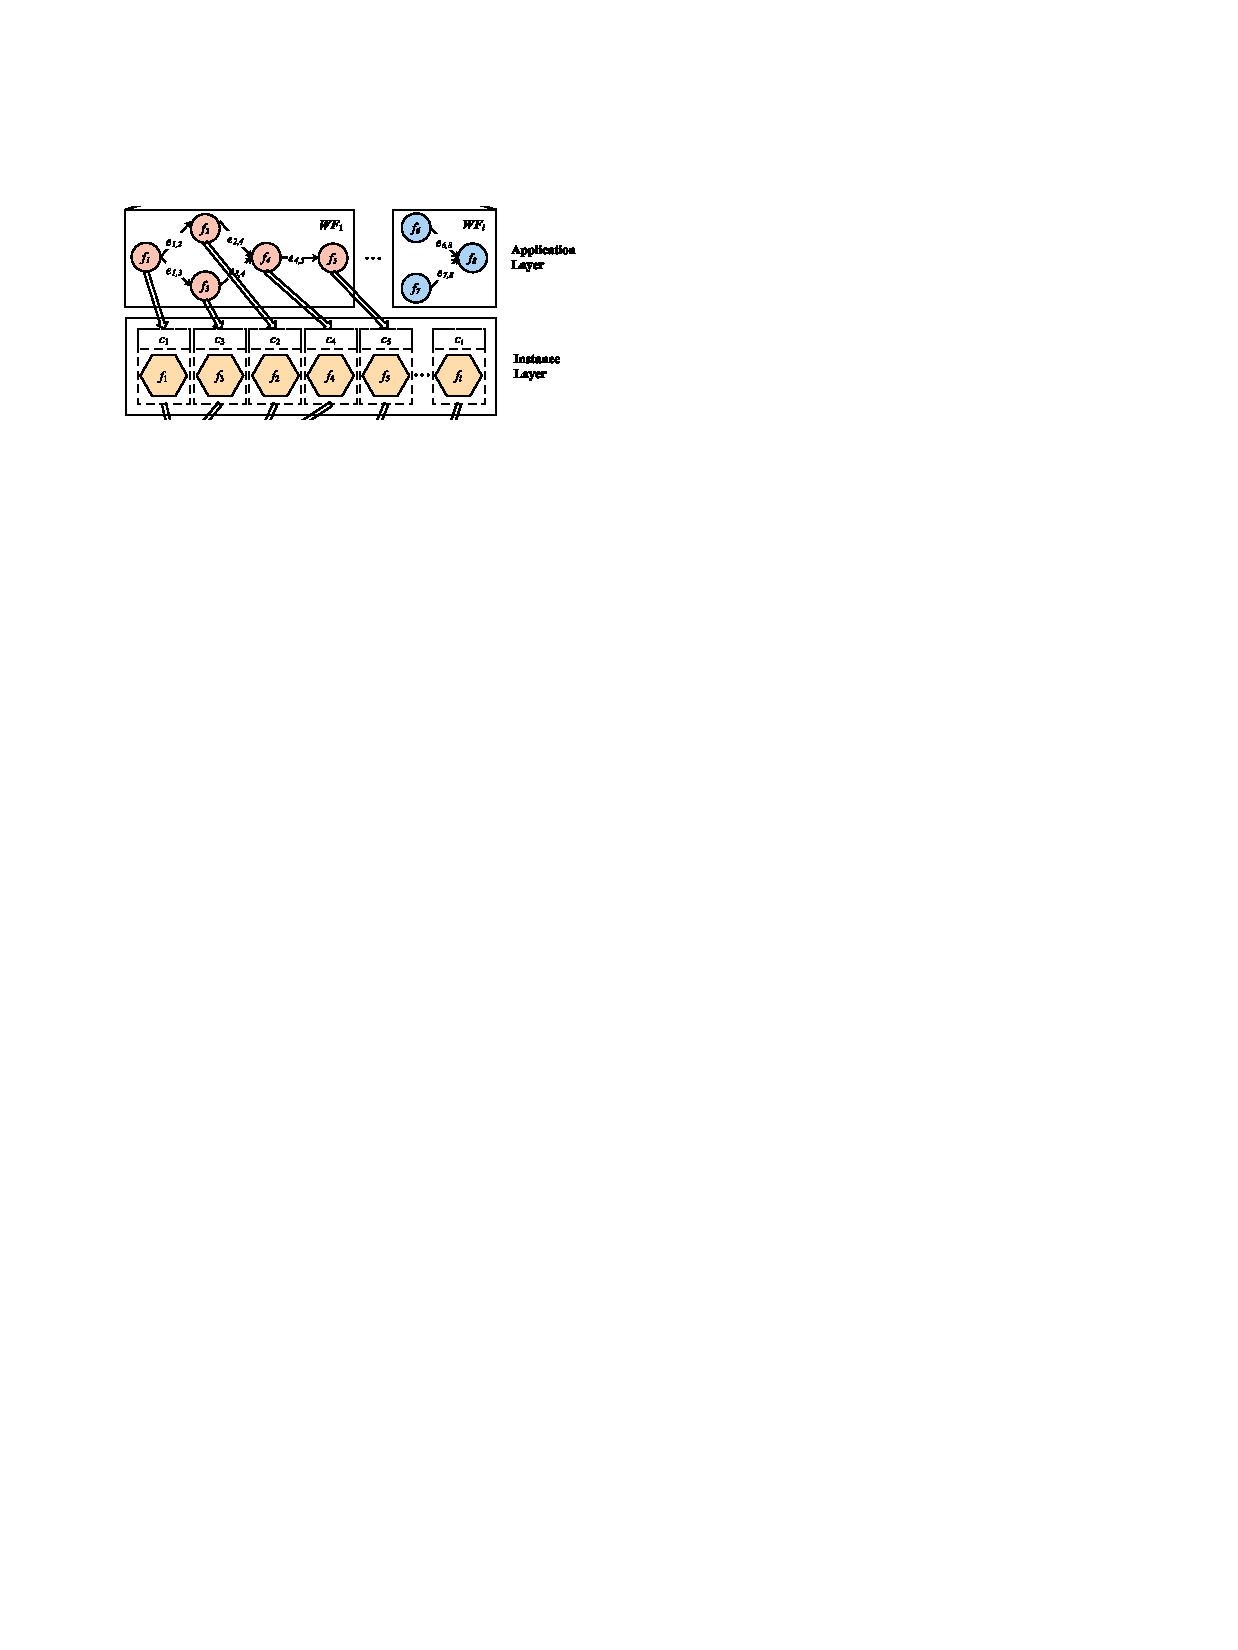
\includegraphics[height=0.5\textheight]{img/serverless-system-architecture/system-model-instance.pdf}
  \end{figure}

  工作流中的每一个函数都会被分配到一个 runtime 匹配的容器中执行。运行不同语言的函数所需要的容器镜像各不相同\footnote{\url{https://hub.docker.com/search?q=openwhisk\%2Faction}}。当函数被调用时,创建容器;当函数执行完毕时释放容器。

  运行函数的容器通常被称为函数实例 (Function Instance) 或 Pod (Kubernetes 中的概念)。
\end{frame}

\begin{frame}{无服务器计算系统结构}{Server Layer}
  \begin{columns}
    \column{0.49\textwidth}
    \begin{figure}
      \centering
      \includegraphics[width=\textwidth]{img/serverless-system-architecture/system-model-server.pdf}
    \end{figure}
    函数实例 $c$ 被分配到物理机服务器 $s$ 上的某一个非一致性内存访问 (Non-Uniform Memory Access, NUMA) 节点 $nn$ 上执行。

    \column{0.02\textwidth}
    \rule{0.2mm}{0.825\textheight}

    \pause

    \column{0.49\textwidth}
    \begin{figure}
      \centering
      \includegraphics[height=0.5\textheight]{img/serverless-system-architecture/NUMA-nodes.png}
    \end{figure}
    NUMA 架构常见于双路 CPU 服务器主板中,每个 CPU 都有专用的内存 (因此称为非一致性内存访问) 。两节点之间通过高速通道进行数据传输。
  \end{columns}
\end{frame}

% -------------------------------------------------------- %
\section{研究现状与主要贡献}
% -------------------------------------------------------- %

\begin{frame}{研究现状与主要贡献}{Inaccurate and Inefficient Resource Configuration Estimation}
  \begin{columns}
    \column{0.45\textwidth}
    现状:
    \begin{itemize}
      \item 使用实验室测试、简单统计、人工经验或穷举法估计资源配置,会因为忽视运行日志而导致在动态、异构场景下供需不匹配。
      \item 使用历史或现场日志的资源配置估计方法均针对同构服务器或应用,并且假设日志数据充足;然而现场日志收集效率低下,需要等待较长时间。
    \end{itemize}

    \column{0.45\textwidth}
    贡献:
    \begin{itemize}
      \item 提出一种工作流资源配置估计方法
      \item 使用随机森林构建多任务专家分类器
      \item 识别服务器类型和资源容量之间的耦合关系
    \end{itemize}
  \end{columns}
\end{frame}

\begin{frame}{研究现状与主要贡献}{High-Latency Indirect Communication Way between Functions}
  \begin{columns}
    \column{0.45\textwidth}
    现状:
    \begin{itemize}
      \item 数据密集型应用对 NUMA 架构中的通信延迟十分敏感,但这个问题常常被忽视
      \item 现有的考虑函数间通信来优化工作流执行时间的方法,仅使用外部存储作为通信媒介,或者没有考虑其他通信媒介
    \end{itemize}

    \column{0.45\textwidth}
    贡献:
    \begin{itemize}
      \item 提出了一种时空联合的函数实例分配方法
      \item 考虑了函数分配的优先级、函数间通信的亲和度以及服务器的 NUMA 架构
      \item 考虑了三种通信媒介,使用启发式算法完成函数到容器的分配
    \end{itemize}
  \end{columns}
\end{frame}

\begin{frame}{研究现状与主要贡献}{Long Resource Readiness Time Due to Passive Server Scaling}
  \begin{columns}
    \column{0.45\textwidth}
    现状:
    \begin{itemize}
      \item 大多数服务器弹性伸缩方法都假设服务器一直处于可用状态,或被动扩展服务器,导致资源准备时间过长
      \item 使用基于回归的方法 (如:ARIMA 和 LSTM) 来预测请求到达情况,都使用连续数值,无法捕获特定时间段的突变
      \item 剧烈波动的请求到达情况容易导致高估或低估的出现
    \end{itemize}

    \column{0.45\textwidth}
    贡献:
    \begin{itemize}
      \item 提出了一种主动服务器弹性扩展方法
      \item 使用融合的 GRU (RNN的一种) 模型来预测工作负载模式,包括负载水平、趋势、幅度等特征
      \item 该方法动态分配注意力权重来指导弹性伸缩决策,从而应对多变的工作负载模式
    \end{itemize}
  \end{columns}
\end{frame}

% -------------------------------------------------------- %
\section{问题表述}
% -------------------------------------------------------- %

\begin{frame}{问题表述}
  本文需要获得以下三种方案:
  \begin{itemize}
    \item 应用配置方案 (Application Configuration Scheme)
    \item 实例分配方案 (Instance Allocation Scheme)
    \item 服务器扩缩容方案 (Server Scaling Scheme)
  \end{itemize}
\end{frame}

\begin{frame}{问题表述}{Application Configuration Scheme}
  应用配置方案 (Application Configuration Scheme) $M$:
  \begin{equation*}
    M = \{m_{p,c,r}|m_{p,c,r} = (WF_p,SC_c,RC_r)\}
  \end{equation*}
  \begin{itemize}
    \item 给定第 $p$ 个工作流 $WF_p$ 确定最合适的第 $c$ 种服务器类型 $SC_c$ 和第 $r$ 个资源容量配置 $RC_r$ 。
  \end{itemize}
\end{frame}

\begin{frame}{问题表述}{Instance Allocation Scheme}
  实例分配方案 (Instance Allocation Scheme) $N$:
  \begin{align*}
    N = \{&n_{i,j,x}|n_{i,j,x} = (c_i,nn_j,s_x,G(f_i),SST(f_i),SFT(f_i)), \\
    &c_i \leftarrow f_i,f_i \in WF_p, \text{and} \, nn_j \in NS(s_x)\}
  \end{align*}
  \begin{itemize}
    \item 将第 $i$ 个函数实例 $c_i$ 分配到第 $x$ 个服务器 $s_x$ 中的第 $j$ 个 NUMA 节点 $nn_j$ 上。
    \item 函数 $f_i$ 要在服务开始时间 $SST(f_i)$ 到服务结束时间 $SFT(f_i)$ 内占据资源容量 $G(f_i)$ 。
    \item $NS(s_x)$ 是服务器 $s_x$ 的 NUMA 节点集合。
  \end{itemize}
\end{frame}

\begin{frame}{问题表述}{Server Scaling Scheme}
  服务器扩缩容方案 (Server Scaling Scheme) $O$:
  \begin{align*}
    O_1 &= \{o_{c,T^\prime}|o_{c,T^\prime} = (SC_c,N_{c,T^\prime})\} \\
    O_2 &= \{o_{x,a}|o_{x,a} = (s_x,a)\}
  \end{align*}
  $O$ 包含扩容方案 $O_1$ 和缩容方案 $O_2$:
  \begin{itemize}
    \item $O_1$: 在每个扩缩容周期 $T^\prime$ 中,每一种服务器类型 $SC_c$ 需要启动的服务器数量 $N_{c,T^\prime}$ 。
    \item $O_2$: 每一台服务器 $s_x$ 在租期到期时,是否释放;$a=0$ 表示释放该服务器,$a=1$ 表示保留该服务器并继续租用。
  \end{itemize}
\end{frame}

\begin{frame}{问题表述}{优化目标}\label{label:objective}
  在确保每一个应用执行的满意度的前提下,最小化从云服务提供商 (Cloud Service Provider, CSP) 租用服务器的总成本:
  \begin{gather*}
    \min cost \\
    \text{s.t. } score_{WF_p} \geqslant T_{score}, \forall WF_p
  \end{gather*}
  \begin{itemize}
    \item $cost$: FaaS 服务提供者租用服务器的总成本
    \item $score_{WF_p}$: 在特定的资源分配结果下,应用工作流的执行满意度得分
    \item $T_{score}$: 应用工作流的执行满意度阈值
  \end{itemize}

  $T_{score}$ 默认设置为最大值 $100$ ,表示要求完全满足工作流的 QoS 需求;$T_{score}$ 越低,表示对工作流的 QoS 要求越低。

  \hfill\hyperlink{label:bet-and-bec}{\beamerbutton{Back to AllocationSatisfactionModel}}
\end{frame}

% -------------------------------------------------------- %
\section{方法描述}
% -------------------------------------------------------- %

\subsection{Overview}

\begin{frame}{Overview}{PLOEA}
  本文提出的方法为“基于异构性感知的无服务器应用主动弹性资源分配”方法。取名为 PLOEA:

  \begin{center}
    heterogeneity-aware \textbf{\textcolor{NCEPUblue}{P}}roactive server\textbf{\textcolor{NCEPUblue}{L}}ess w\textbf{\textcolor{NCEPUblue}{O}}rkflow \textbf{\textcolor{NCEPUblue}{E}}lastic \textbf{\textcolor{NCEPUblue}{A}}llocation method
  \end{center}
\end{frame}

\begin{frame}{Overview}{PLOEA 系统架构}
  \begin{figure}
    \centering
    \includegraphics[height=0.8\textheight]{img/method/PLOEA-system.pdf}
  \end{figure}
\end{frame}

\begin{frame}{Overview}{PLOEA 系统架构}
  \begin{columns}
    \column{0.5\textwidth}
    \begin{figure}
      \centering
      \includegraphics[height=0.8\textheight]{img/method/PLOEA-system-left.pdf}
    \end{figure}

    \column{0.5\textwidth}
    PLOEA 系统包含三个数据库:
    \begin{itemize}
      \item \textit{Workflow Traces Database} \\
        记录应用工作流的静态信息
      \item \textit{Execution Logs Database} \\
        记录应用工作流执行时的日志数据,包括:执行时间、开销和资源使用情况
      \item \textit{Workload Traces Database} \\
        记录工作负载信息,包括请求到达情况、负载变化趋势及幅度
    \end{itemize}
  \end{columns}
\end{frame}

\begin{frame}{Overview}{PLOEA 系统架构}\label{label:architecture-1}
  \begin{columns}
    \column{0.45\textwidth}
    \begin{figure}
      \centering
      \includegraphics[height=0.75\textheight]{img/method/PLOEA-system-right.pdf}
    \end{figure}

    \column{0.55\textwidth}
    PLOEA 系统包含四个模块:
    \begin{enumerate}
      \item \hyperlink{label:application-need-analyzer}{\underline{\textit{Application Need Analyzer}}} \\
        根据 \textit{Workflow Traces Database} 中的数据,分析应用的执行需求,选择合适的满意度模型
      \item \hyperlink{label:resource-configuration-estimator}{\underline{\textit{Resource Configuration Estimator}}} \\
        基于 \textit{Execution Logs Database} 构建一个本地专家分类器,用于估计每一个应用工作流的最优资源配置,用于指导函数实例的分配
    \end{enumerate}
  \end{columns}
\end{frame}

\begin{frame}{Overview}{PLOEA 系统架构}\label{label:architecture-2}
  \begin{columns}
    \column{0.45\textwidth}
    \begin{figure}
      \centering
      \includegraphics[height=0.75\textheight]{img/method/PLOEA-system-right.pdf}
    \end{figure}

    \column{0.55\textwidth}
    PLOEA 系统包含四个模块:
    \begin{enumerate}
        \setcounter{enumi}{2}
      \item \hyperlink{label:spatiotemporal-joint-instance-allocator}{\underline{\textit{Spatiotemporal Joint Instance Allocator}}} \\
        获取 \textit{Workflow Traces Database} 中的 DAG 信息,根据函数的分配优先级和通信亲和度,对函数进行分组、排序后,将函数实例分配到 NUMA 节点上
      \item \hyperlink{label:proactive-server-elastic-scaler}{\underline{\textit{Proactive Server Elastic Scaler}}} \\
        从 \textit{Workload Traces Database} 中获取此次扩缩容周期 $T^\prime$ 内的工作负载信息,用来预测下一周期 $T^\prime + 1$ 的工作负载情况,根据预测结果和资源使用情况对服务器进行扩缩容
    \end{enumerate}
  \end{columns}
\end{frame}

\subsection{Application Need Analyzer}

\begin{frame}{Application Need Analyzer}\label{label:application-need-analyzer}
  \begin{columns}
    \column{0.4\textwidth}
    \begin{figure}
      \centering
      \includegraphics[scale=1.5]{img/method/application-need-analyzer.pdf}
    \end{figure}

    \column{0.6\textwidth}
    Application Need Analyzer 包含两部分内容:
    \begin{itemize}
      \item Application Representation Model: 无服务器应用数学模型
      \item Allocation Satisfaction Model: 满意度模型
    \end{itemize}
  \end{columns}
  \hfill\hyperlink{label:architecture-1}{\beamerbutton{Back to PLORA System Architecture}}
\end{frame}

\begin{frame}{Application Need Analyzer}{Application Representation Model}\label{label:functional-attributes}
  为了描述无服务器应用的执行需求,方便估计资源配置,本文构建的无服务器应用数学模型包括\textbf{与功能相关的属性}和\textbf{与函数无关的属性}。这些属性由应用开发者设置或由 CSP 推荐。

  \vfill

  与功能相关的属性 (functional attributes) $FA$ 定义为:
  \begin{equation*}
    FA = \{Name, DAG, PZ, FZ\}
  \end{equation*}
  \begin{itemize}
    \item $Name$: 应用 $WF_p$ 的名称
    \item $DAG$: 应用 $WF_p$ 的函数执行逻辑和数据传输关系
    \item $PZ$: 应用 $WF_p$ 的问题规模 (Problem Size) ,表示应用的输入参数规模
    \item $FZ$: 应用 $WF_p$ 的文件大小 (File Size) ,表示应用输入的数据文件大小
  \end{itemize}
  \hfill\hyperlink{label:sample-representation}{\beamerbutton{Back to ResourceConfigurationEstimator}}
\end{frame}

\begin{frame}{Application Need Analyzer}{Application Representation Model}\label{label:non-functional-attributes}
  与功能无关的属性 (non-functional attributes) $NFA$ 定义为:
  \begin{equation*}
    NFA = \{SST, SFT, EET, DET, EEC, DEC, PRE\}
  \end{equation*}
  \begin{itemize}
    \item $SST$: $WF_p$ 的服务开始时间 (Service Start Time) ,用于确定应用立即执行或推迟执行
    \item $SFT$: $WF_p$ 的服务结束时间 (Service Finish Time) ,与 $SST$ 求差可得应用的执行时间
    \item $EET$: $WF_p$ 的期待执行时间 (Expected Execution Time) ,是应用执行时间的软限制
    \item $DET$: $WF_p$ 的最大执行时间 (Dead Execution Time) ,是应用执行时间的硬限制
    \item $EEC$: $WF_p$ 的期望执行成本 (Expected Execution Cost) ,是应用执行成本的软限制
    \item $DEC$: $WF_p$ 的最大执行成本 (Dead Execution Cost) ,是应用执行成本的硬限制
    \item $PRE$: $WF_p$ 的执行偏好 (Preference) ,在 $\{0,1\}$ 中取值,$0$ 表示偏向于性能,$1$ 表示偏向于节约成本
  \end{itemize}
  \hfill\hyperlink{label:sample-representation}{\beamerbutton{Back to ResourceConfigurationEstimator}}
\end{frame}

\begin{frame}{Application Need Analyzer}{Allocation Satisfaction Model}
  现有的研究对于满意度的考量主要集中于应用执行的最后期限 (deadline) 。本文提出的满意度指标同时考虑了应用执行的性能和成本,用于指导资源分配。
  \pause
  \begin{definition}
    对于一个应用 $WF_p$ ,其满意度 $score_{WF_p}$ 定义为:
    \begin{equation*}
      score_{WF_p} = \alpha \cdot score_{WF_p}^{perf} + (1-\alpha) \cdot score_{WF_p}^{cost}
    \end{equation*}
    其中:
    \begin{itemize}
      \item $score_{WF_p}^{perf}$: 应用 $WF_p$ 的性能满意度 (performance satisfaction score)
      \item $score_{WF_p}^{cost}$: 应用 $WF_p$ 的成本满意度 (cost satisfaction score)
      \item $\alpha$: CSP 指定的权重系数,默认为 $0.5$ 。
    \end{itemize}
  \end{definition}
\end{frame}

\begin{frame}{Application Need Analyzer}{Allocation Satisfaction Model}
  $score_{WF_p}^{perf}$ 和 $score_{WF_p}^{cost}$ 如下图所示:
  \begin{figure}
    \centering
    \includegraphics[height=0.5\textheight]{img/method/satisfaction-model.pdf}
  \end{figure}
  其中:
  \begin{itemize}
    \item $AET$: 应用 $WF_p$ 的实际执行时间 (Actual Execution Time)
    \item $AEC$: 应用 $WF_p$ 的实际执行成本 (Actual Execution Cost)
  \end{itemize}
\end{frame}

\begin{frame}{Application Need Analyzer}{Allocation Satisfaction Model}
  \begin{figure}
    \centering
    \includegraphics[height=0.4\textheight]{img/method/satisfaction-model.pdf}
  \end{figure}
  当 \textcolor{red}{$PRE=0$} 时,执行偏好为\textcolor{red}{性能}优先:
  \begin{equation*}
    score_{WF_p}^{perf} =
    \begin{cases}
      100, & \text{if } AET \leqslant EET \\
      100 \cdot \frac{AET - DET}{EET - DET}, & \text{if } EET < AET < DET \\
      0, & \text{if } AET \geqslant DET
    \end{cases}
  \end{equation*}
\end{frame}

\begin{frame}{Application Need Analyzer}{Allocation Satisfaction Model}
  \begin{figure}
    \centering
    \includegraphics[height=0.4\textheight]{img/method/satisfaction-model.pdf}
  \end{figure}
  当 \textcolor{red}{$PRE=0$} 时,执行偏好为\textcolor{red}{性能}优先:
  \begin{equation*}
    score_{WF_p}^{cost} =
    \begin{cases}
      100, & \text{if } AEC \leqslant EEC \\
      (100-S_{th}) \cdot \frac{AEC - DEC}{EEC - DEC} + S_{th}, & \text{if } EEC < AEC < DEC \\
      0, & \text{if } AEC \geqslant DEC
    \end{cases}
  \end{equation*}
  其中 $S_{th}>0$ 是成本满意度的阈值(最低值)。
\end{frame}

\begin{frame}{Application Need Analyzer}{Allocation Satisfaction Model}
  \begin{figure}
    \centering
    \includegraphics[height=0.4\textheight]{img/method/satisfaction-model.pdf}
  \end{figure}
  当 \textcolor{blue}{$PRE=1$} 时,执行偏好为\textcolor{blue}{成本}优先:
  \begin{equation*}
    score_{WF_p}^{cost} =
    \begin{cases}
      100, & \text{if } AEC \leqslant EEC \\
      100 \cdot \frac{AEC - DEC}{EEC - DEC}, & \text{if } EEC < AEC < DEC \\
      0, & \text{if } AEC \geqslant DEC
    \end{cases}
  \end{equation*}
\end{frame}

\begin{frame}{Application Need Analyzer}{Allocation Satisfaction Model}
  \begin{figure}
    \centering
    \includegraphics[height=0.4\textheight]{img/method/satisfaction-model.pdf}
  \end{figure}
  当 \textcolor{blue}{$PRE=1$} 时,执行偏好为\textcolor{blue}{成本}优先:
  \begin{equation*}
    score_{WF_p}^{pref} =
    \begin{cases}
      100, & \text{if } AET \leqslant EET \\
      (100-S_{th}) \cdot \frac{AET - DET}{EET - DET} + S_{th}, & \text{if } EET < AET < DET \\
      0, & \text{if } AET \geqslant DET
    \end{cases}
  \end{equation*}
  其中 $S_{th}>0$ 是性能满意度的阈值(最低值)。
\end{frame}

\begin{frame}{Application Need Analyzer}{Allocation Satisfaction Model}\label{label:bet-and-bec}
  \begin{figure}
    \centering
    \includegraphics[height=0.5\textheight]{img/method/satisfaction-model.pdf}
  \end{figure}
  令 $score_{WF_p}^{perf} = T_{score}$ 和 $score_{WF_p}^{cost} = T_{score}$ ,分别得到应用 $WF_p$ 的最优执行时间 $BET$ (Best Execution Time) 和最优执行成本 $BEC$ (Best Execution Cost) 。其中,$T_{score}$ 为\hyperlink{label:objective}{\underline{优化目标}}中需要满足的阈值。$BET$ 和 $BEC$ 在后续模块中会使用到。

  \hfill\hyperlink{label:sample-representation}{\beamerbutton{Back to ResourceConfigurationEstimator}}
\end{frame}

\subsection{Resource Configuration Estimator}

\begin{frame}{Resource Configuration Estimator}\label{label:resource-configuration-estimator}
  \begin{columns}
    \column{0.4\textwidth}
    \begin{figure}
      \centering
      \includegraphics[scale=1.5]{img/method/resource-configuration-estimator.pdf}
    \end{figure}

    \column{0.6\textwidth}
    微服务架构广泛应用于应用开发中,其中应用调用的函数大部分是复用的,并且拥有相似的资源使用情况。因此可以通过分析应用的执行日志来估计应用的资源需求。

    Resource Configuration Estimator 包含两部分内容:
    \begin{itemize}
      \item 无服务器应用资源配置模型
      \item 专家分类器的构建与训练
    \end{itemize}
  \end{columns}
  \hfill\hyperlink{label:architecture-1}{\beamerbutton{Back to PLORA System Architecture}}
\end{frame}

\begin{frame}{Resource Configuration Estimator}{无服务器应用资源配置模型}
  无服务器应用的资源配置 $R(WF_p)$ 包含两个因子:
  \begin{equation*}
    R(WF_p) = \{SC, RC\}
  \end{equation*}
  \begin{itemize}
    \item $SC$: 服务器类型。不同类型的服务器拥有不同的处理速度和价格。\textbf{同一个工作流中的函数倾向于使用同一种类型的服务器}。若一共有 $m$ 种服务器类型,则服务器类型的集合: \[SC = \{SC_1,SC_2, \dots ,SC_m\}\]
    \item $RC$: 资源容量。每个函数都有其可用的资源范围,拥有资源多的函数性能更好,执行速度更快。将资源容量的范围离散化为 $n$ 个等级,则可选资源容量的集合: \[RC = \{RC_1,RC_2, \dots ,RC_n\}\] \[RC_i = \{R_i^{f_1}, R_i^{f2}, \dots ,R_i^{f_{|WF_p|}}\}, (1 \leqslant i \leqslant n)\] 其中,$|WF_p|$ 是工作流 $WF_p$ 中的函数数量,$R_i^{f_j}$ 表示函数 $f_j$ 拥有的资源容量。
  \end{itemize}
\end{frame}

\begin{frame}{Resource Configuration Estimator}{专家分类器的构建与训练——source application}
  分类器的训练往往需要大量的数据,但有时候 \textit{Execution Logs Database} 中存储的 $WF_p$ 的日志数据很少甚至没有。因此,我们可以通过分析与 $WF_p$ 相似的工作流的日志数据来估计 $WF_p$ 的资源使用情况。与 $WF_p$ 相似的工作流被称为 \textit{source application} 。
\end{frame}

\begin{frame}{Resource Configuration Estimator}{专家分类器的构建与训练——source application}
  筛选 source application 的第一步 \textit{Initial screening}:

  \pause

  通过计算 $WF_p$ 与候选工作流 $WF_c$ 静态指标之间的\textbf{静态相似度} $S(WF_p,WF_c)$ 来筛选 source application 。静态指标包括应用本身,以及与其执行相关的容器实例和服务器的指标。如下表所示:
  \begin{table}
    \centering
    \resizebox{\textwidth}{!}{
      \begin{tabular}{cclccl}
        \toprule
        Category & Feature & Description & Category & Feature & Description\\
        \midrule
        \multirow{4}{*}{Application} & \textit{CodeInfo} & 代码信息或 DAG & \multirow{4}{*}{Server} & \textit{ServerType} & 服务器类型\\
        & \textit{InputPara} & 输入参数 & & \textit{Hardware} & 服务器硬件类型\\
        & \textit{InputFile} & 输入文件 & & \textit{Software} & 服务器软件类型\\
        & \textit{AppType} & 资源需求类型 & & \textit{ResCap} & 服务器资源容量\\
        \midrule
        \multirow{3}{*}{Instance} & \textit{ImageInfo} & 容器镜像信息 \\
        & \textit{InstanceType} & 函数实例类型 \\
        & \textit{ResAlloc} & 资源请求容量 \\
        \bottomrule
    \end{tabular}}
  \end{table}
\end{frame}

\begin{frame}{Resource Configuration Estimator}{专家分类器的构建与训练——source application}
  被选为 source application 的候选工作流 $WF_c$ 满足以下两个限制条件:
  \begin{gather*}
    \begin{cases}
      S(WF_p,WF_c) \geqslant T^s, \text{s.t. } S(WF_p,WF_c) = \sum_{i=1}^{N_m} w_i \cdot sim_i \\
      N_{WF_c} \geqslant T^n
    \end{cases} \\
    sim_i =
    \begin{cases}
      1, & \text{if } m_i^{WF_p} \text{ is similar to } m_i^{WF_c} \\
      0, & \text{otherwise}
    \end{cases}
  \end{gather*}
  \begin{columns}
    \column{0.5\textwidth}
    \begin{itemize}
      \item $S(WF_p,WF_c)$: $WF_p$ 与 $WF_c$ 的相似度
      \item $T^s$: 选中 $WF_c$ 的静态相似度阈值
      \item $N_m$: 静态指标的数量
      \item $w_i$: 第 $i$ 个静态指标的权重
    \end{itemize}

    \column{0.5\textwidth}
    \begin{itemize}
      \item $m_i^{WF_p}$: $WF_p$ 的第 $i$ 个静态指标
      \item $m_i^{WF_c}$: $WF_c$ 的第 $i$ 个静态指标
      \item $N_{WF_c}$: $WF_c$ 的日志数量
      \item $T^n$: 日志数量阈值
    \end{itemize}
  \end{columns}
\end{frame}

\begin{frame}{Resource Configuration Estimator}{专家分类器的构建与训练——source application}
  筛选 source application 的第二步 \textit{Fine screening}:

  \pause

  如果 \textit{Execution Logs Database} 中储存了少量 $WF_p$ 的日志数据,那么可以使用这些动态数据来计算 $WF_p$ 与 $WF_c$ 之间的\textbf{动态相似度} $D(WF_p,WF_c)$ 。满足以下条件的可以被选为 source application :
  \begin{equation*}
    D(WF_p,WF_c) \geqslant T^d, \text{s.t. } D(WF_p,WF_c) = \frac{sv_p \cdot sv_c}{||sv_p|| \cdot ||sv_c||}
  \end{equation*}
  $D(WF_p,WF_c)$ 使用余弦相似度定义,其中 $sv_p$ 和 $sv_c$ 分别是 $WF_p$ 和 $WF_c$ 的 \textit{simple vector} ,$T^d$ 为选中 $WF_c$ 的动态相似度阈值。
  \begin{equation*}
    sv = (fv, rv)
  \end{equation*}
  $sv$ 向量包含两部分:\textit{feature vector} $fv$ 和 \textit{configuration vector} $rv$ 。前者来自于 \textit{Workflow Traces Database} 中的静态信息,后者来自于 \textit{Execution Logs Database} 中的日志数据。
\end{frame}

\begin{frame}{Resource Configuration Estimator}{专家分类器的构建与训练——ensemble resource configuration estimation model}
  专家分类器使用集成学习中的\textbf{随机森林 (RF)} 算法来估计 $WF_p$ 的资源配置。首先使用 \textit{Workflow Traces Database} 中\textbf{所有应用}的数据训练 RF 模型,然后使用该模型将 $WF_p$ 划分为 $SC$ 集合中的某一类和 $RC$ 集合中的某一类。模型的构建与训练一共包含五个步骤。
  \begin{figure}
    \centering
    \includegraphics[height=0.6\textheight]{img/method/resource-configuration-estimation-model.pdf}
  \end{figure}
\end{frame}

\begin{frame}{Resource Configuration Estimator}{专家分类器的构建与训练——Step 1: Sample representation}\label{label:sample-representation}
  \begin{figure}
    \centering
    \includegraphics[height=0.4\textheight]{img/method/resource-configuration-estimation-model.pdf}
  \end{figure}
  \textit{Workflow Traces Database} 中的所有应用都使用如下特征向量表示:
  \begin{equation*}
    fv = [DAG, PZ, FZ, BET, BEC, PRE]
  \end{equation*}
  其中,$DAG$, $PZ$, $FZ$ 为 \hyperlink{label:functional-attributes}{\underline{functional attributes}} ,$PRE$ 为 \hyperlink{label:non-functional-attributes}{\underline{non-functional attributes}} 中的执行偏好,$BET$ 和 $BEC$ 为 \hyperlink{label:bet-and-bec}{\underline{满意度模型}} 中的最优执行时间和最优执行成本。
\end{frame}

\begin{frame}{Resource Configuration Estimator}{专家分类器的构建与训练——Step 2: Model generation}
  \begin{figure}
    \centering
    \includegraphics[height=0.4\textheight]{img/method/resource-configuration-estimation-model.pdf}
  \end{figure}
  使用 \textit{Workflow Traces Database} 中的数据 $fv$ 训练 RF 模型,目标函数为:
  \begin{equation*}
    \max_{f,t} w G_s + (1-w) G_r, \text{s.t. } 0 \leqslant w \leqslant 1
  \end{equation*}
  其中,$G_s$ 和 $G_r$ 分别是 $fv$ 在 $SC$ 和 $RC$ 两个分类任务中各自的信息增益;$f$ 和 $t$ 分别是决策树中非叶子节点的特征和阈值;$w$ 是权重系数。

  训练好的 RF 模型可以对给定的应用 $WF_p$ 在 $SC$ 和 $RC$ 两个维度上进行分类。
\end{frame}

\begin{frame}{Resource Configuration Estimator}{专家分类器的构建与训练——Step 3: Model estimation}
  \begin{columns}
    \column{0.45\textwidth}
    \begin{figure}
      \centering
      \includegraphics[width=\textwidth]{img/method/resource-configuration-estimation-model.pdf}
    \end{figure}

    \column{0.55\textwidth}
    给定应用 $WF_p$ 及其特征向量 $fv$ ,
    \begin{itemize}
      \item<1-> 如果 $WF_p$ 的日志数据足够,则直接通过 RF 模型确定 $WF_p$ 的服务器配置 $SC_i$ 和资源配置 $RC_j$ ;
      \item<2-> 如果完全没有 $WF_p$ 的日志数据,则使用 RF 对 source application 中总计 $N$ 个应用进行分类,得到 Common Models 结果 $[R_1^C, R_2^C, \dots, R_N^C]$
      \item<3-> 如果存在少量 $WF_p$ 的日志数据,则使用这些单独训练一个 RF Individual Model ,并对 $fv$ 进行分类,得到结果 $R^I$
    \end{itemize}
    \uncover<4->{最终得到分类结果 $Rs_p = [R_1^C, R_2^C, \dots, R_N^C, R^I]$ 。}
  \end{columns}
\end{frame}

\begin{frame}{Resource Configuration Estimator}{专家分类器的构建与训练——Step 4: Voting output}
  \begin{figure}
    \centering
    \includegraphics[height=0.4\textheight]{img/method/resource-configuration-estimation-model.pdf}
  \end{figure}
  基于 $N+1$ 个分类结果 $Rs_p = [R_1^C, R_2^C, \dots, R_N^C, R^I]$ ,使用投票机制\footnote{\footnotesize 投票机制文中未详细给出}来确定 $WF_p$ 的最优资源配置 $R(WF_p)$ 。
\end{frame}

\begin{frame}{Resource Configuration Estimator}{专家分类器的构建与训练——Step 5: Model regeneration}
  \begin{figure}
    \centering
    \includegraphics[height=0.4\textheight]{img/method/resource-configuration-estimation-model.pdf}
  \end{figure}
  当出现如下两种情况时,PLOEA 会收集现场日志数据,重新训练 RF 模型:
  \begin{itemize}
    \item 由于系统此前从未遇到过相似的应用,导致找不到与 $WF_p$ 相似的 source application
    \item 由于应用的资源使用模式发生了改变,导致 RF 模型估计资源配置的误差无法接受
  \end{itemize}
\end{frame}

\subsection{Spatiotemporal Joint Instance Allocator}

\begin{frame}{Spatiotemporal Joint Instance Allocator}\label{label:spatiotemporal-joint-instance-allocator}
  \begin{columns}
    \column{0.4\textwidth}
    \begin{figure}
      \centering
      \includegraphics[scale=1.4]{img/method/spatiotemporal-joint-instance-allocator.pdf}
    \end{figure}

    \column{0.6\textwidth}
    Spatiotemporal Joint Instance Allocator 包含三部分内容:
    \begin{itemize}
      \item Three-Tier Inter-Instance Communication Media: 函数实例三层通信模型
      \item The Function Grouping and Checking: 函数分组策略
      \item The Instance Joint Allocation: 函数实例分配方法
    \end{itemize}
  \end{columns}
  \hfill\hyperlink{label:architecture-2}{\beamerbutton{Back to PLORA System Architecture}}
\end{frame}

\begin{frame}{Spatiotemporal Joint Instance Allocator}{Three-Tier Inter-Instance Communication Media}
  目前主流服务器均采用 NUMA 架构,如图所示:
  \begin{figure}
    \centering
    \includegraphics[height=0.5\textheight]{img/method/numa-architecture.pdf}
  \end{figure}
  结合 NUMA 架构,本文使用三种函数实例间的通信模型:
  \begin{itemize}
    \item 位于同一 NUMA 节点的函数实例通过\textbf{三级缓存}进行通信
    \item 位于同一服务器不同 NUMA 节点的函数实例通过节点内存间的高速通道进行通信
    \item 位于不同服务器的函数实例通过网络进行通信
  \end{itemize}
\end{frame}

\begin{frame}{Spatiotemporal Joint Instance Allocator}{The Function Grouping and Checking}
  应用工作流 $WF_p$ 只有在其所有函数实例都部署完毕后才能开始执行。因此,工作流中的函数 $f_i$ 的最早服务开始时间 (Earliest Service Start Time) $ESST$ 和最早服务结束时间 (Earliest Service Finish Time) $ESFT$ 为:
  \begin{align*}
    ESST(f_i,c_i,T) &= \max_{f_i \in WF_p} \{T + IT(c_i)\} \\
    ESFT(f_i,c_i,T) &= ESST(f_i,c_i,T) + CST
  \end{align*}
  其中,$T$ 为当前时间,$IT(c_i)$ 为容器 $c_i$ 的初始化时间,$CST$ 为工作流服务开始到服务结束持续的时间,即:$CST = SFT - SST$ 。
\end{frame}

\begin{frame}{Spatiotemporal Joint Instance Allocator}{The Function Grouping and Checking}
  容器初始化时间 $IT(c_i)$ 有以下三种可能的取值:
  \begin{equation*}
    IT(c_i) =
    \begin{cases}
      CT(c_i), & \text{cached images} \\
      CT(c_i) + PT(c_i), & \text{no images} \\
      CT(c_i) + PT(c_i) + CT(s_x), & \text{new server}
    \end{cases}
  \end{equation*}
  \begin{enumerate}
    \item 如果容器 $c_i$ 的镜像已经缓存到服务器中,则只需要等待实例的冷启动时间 $CT(c_i)$
    \item 如果服务器本地没有缓存容器 $c_i$ 的镜像,则还需要等待容器拉取的时间 $PT(c_i)$
    \item 如果服务器 $s_x$ 是通过弹性扩展新创建的,则还需要等待服务器的冷启动时间 $CT(s_x)$
  \end{enumerate}
\end{frame}

\begin{frame}{Spatiotemporal Joint Instance Allocator}{The Function Grouping and Checking---Function attribute calculation}
  为了指导函数实例的资源分配,需要计算函数的一些属性:
  \begin{itemize}
    \item 最优次完成时间 (Best sub-finish time) $BFT(f_i)$
    \item 最优次执行成本 (Best sub-execution cost) $BEC(f_i)$
    \item 最早执行开始时间 (Earliest execution start time) $EEST(f_i)$
    \item 最早执行结束时间 (Earliest execution finish time) $EEFT(f_i)$
  \end{itemize}
\end{frame}

\begin{frame}{Spatiotemporal Joint Instance Allocator}{The Function Grouping and Checking---Function attribute calculation}
  最优次完成时间 (Best sub-finish time):
  \begin{gather*}
    BFT(f_i) = BET(WF_p) \times \frac{rank(f_{entry}) - rank(f_i) + ET(f_i)}{rank(f_{entry})} \\
    rank(f_i) = ET(f_i) + \max_{f_s \in succ(f_i)} \{TT(e_{i,s}) + rank(f_s)\}
  \end{gather*}
  \begin{itemize}
    \item $BET(WF_p)$: 工作流 $WF_p$ 的最优执行时间
    \item $rank(f_i)$: 函数节点 $f_i$ 到汇点 $f_{exit}$ 所经历的最长时间 (类似于关键路径的权重)
    \item $ET(f_i)$: 函数 $f_i$ 的执行时间
    \item $succ(f_i)$: 函数 $f_i$ 的所有后继 (successor) 函数集合
    \item $TT(e_{i,s})$: $f_i$ 到 $f_s$ 的数据传输时间
  \end{itemize}
  计算 $ET(f_i)$ 所依据的资源配置是 \textit{Resource Configuration Estimator} 投票得出的最优资源配置 $R(WF_p)$ 。
\end{frame}

\begin{frame}{Spatiotemporal Joint Instance Allocator}{The Function Grouping and Checking---Function attribute calculation}
  最优次执行成本 (Best sub-execution cost):
  \begin{equation*}
    BEC(f_i) = BEC(WF_p) \times \frac{EC(f_i)}{\sum_{f_j \in WF_p} EC(f_j)}
  \end{equation*}
  \begin{itemize}
    \item $EC(f_i)$: 函数 $f_i$ 的执行成本
  \end{itemize}
  计算 $EC(f_i)$ 基于 $WF_p$ 的服务持续时间 $[SST, SFT]$ 和资源配置 $R(WF_p)$ 。
\end{frame}

\begin{frame}{Spatiotemporal Joint Instance Allocator}{The Function Grouping and Checking---Function attribute calculation}
  函数 $f_i$ 在 NUMA 节点 $nn_j$ 上的最早执行开始时间 (Earliest execution start time) 和最早执行结束时间 (Earliest execution finish time):
  \begin{align*}
    EEST(f_i, nn_j) &= \max_{f_p \in pred(f_i)} \{AFT(f_p) + TT(e_{p,i}, nn_j)\} \\
    EEFT(f_i, nn_j) &= EEST(f_i, nn_j) + ET(f_i, nn_j)
  \end{align*}
  \begin{itemize}
    \item $pred(f_i)$: 函数 $f_i$ 的所有前驱 (predecessor) 函数集合
    \item $AFT(f_p)$: 函数 $f_p$ 实际完成时间 (Actual Finish Time)
    \item 函数实例间的通信媒介和服务器的处理速度各不相同,因此 $TT$ 和 $ET$ 均与 NUMA 节点 $nn_j$ 有关
  \end{itemize}
  在实际分配时,为了最小化执行成本并满足应用的性能需求,函数 $f_i$ 不一定会分配到拥有最小 $EEST(f_i, nn_j)$ 的 NUMA 节点上。因此函数执行开始时间 $EST(f_i)$ 大于等于 $EEST(f_i, nn_j)$ 。函数执行结束时间 $EFT(f_i) = EST(f_i) + ET(f_i)$ 。
\end{frame}

\begin{frame}{Spatiotemporal Joint Instance Allocator}{The Function Grouping and Checking---Function grouping}
  假设对如下工作流中的函数进行分组:
  \begin{figure}
    \centering
    \includegraphics[width=\textwidth]{img/method/function-grouping-1.pdf}
  \end{figure}
\end{frame}

\begin{frame}{Spatiotemporal Joint Instance Allocator}{The Function Grouping and Checking---Function grouping}
  第一步:计算所有函数的分配优先级 (allocation urgency) $u_i$:
  \begin{equation*}
    u_i = \frac{BFT(f_i) - TFT(f_i)}{hop(f_i)} \qquad TFT(f_i) = \min_{nn_j \in NS(f_i)} \{EEFT(f_i, nn^{*})\}
  \end{equation*}
  \begin{itemize}
    \item $hop(f_i)$: 从函数 $f_i$ 到汇点 $f_{exit}$ 的关键路径上的函数数量
    \item $TFT(f_i)$: 函数 $f_i$ 的预计完成时间 (Estimated Finish Time)
    \item $NS(f_i)$: 在资源配置为 $R(f_i)$ 的情况下,可以执行函数 $f_i$ 的所有 NUMA 节点集合 (剩余资源无法满足 $R(f_i)$ 的节点不能执行 $f_i$)
  \end{itemize}

  $nn^{*}$ 表示给函数 $f_i$ 分配的 NUMA 节点目前未知,所以假定同一组内的函数通信媒介为“内存间的高速通道”,不同组间的函数通信媒介为“网络”,以此计算 $EEFT$ 。

  $TFT$ 越接近 $BFT$ ,说明函数执行时间超过最优完成时间的风险越高;$hop$ 越大,说明该函数的后继函数越多,对后继函数的延迟影响越大。因此,$u_i$ 越小,说明函数 $f_i$ 越紧急,分配优先级越高。
\end{frame}

\begin{frame}{Spatiotemporal Joint Instance Allocator}{The Function Grouping and Checking---Function grouping}
  假设工作流中所有函数的优先级计算结果如下:
  \begin{figure}
    \centering
    \includegraphics[width=\textwidth]{img/method/function-grouping-2.pdf}
  \end{figure}
\end{frame}

\begin{frame}{Spatiotemporal Joint Instance Allocator}{The Function Grouping and Checking---Function grouping}
  第二步:创建一个新分组 $fg_1$ ,将入度为 $0$ 且 $u_i$ 最小的函数加入分组中并从 DAG 中删除。然后访问其后继函数中 $u_i$ 最小的函数。若该函数入度为 $0$ ,则加入分组并从 DAG 中删除,重复上一句的操作;若该函数入度不为 $0$ ,则停止向 $fg_1$ 中添加函数。
  \begin{figure}
    \centering
    \includegraphics[width=\textwidth]{img/method/function-grouping-3.pdf}
  \end{figure}
\end{frame}

\begin{frame}{Spatiotemporal Joint Instance Allocator}{The Function Grouping and Checking---Function grouping}
  第三步:重复第二步的操作,直到 DAG 中所有函数都被分组。
  \begin{figure}
    \centering
    \includegraphics[width=\textwidth]{img/method/function-grouping-4.pdf}
  \end{figure}
  创建一个新分组 $fg_2$ ,将入度为 $0$ 且 $u_i$ 最小的函数加入分组中并从 DAG 中删除。然后访问其后继函数中 $u_i$ 最小的函数。若该函数入度为 $0$ ,则加入分组并从 DAG 中删除,重复上一句的操作;若该函数入度不为 $0$ ,则停止向 $fg_2$ 中添加函数。
\end{frame}

\begin{frame}{Spatiotemporal Joint Instance Allocator}{The Function Grouping and Checking---Function grouping}
  第三步:重复第二步的操作,直到 DAG 中所有函数都被分组。
  \begin{figure}
    \centering
    \includegraphics[width=\textwidth]{img/method/function-grouping-5.pdf}
  \end{figure}
  创建一个新分组 $fg_3$ ,将入度为 $0$ 且 $u_i$ 最小的函数加入分组中并从 DAG 中删除。然后访问其后继函数中 $u_i$ 最小的函数。若该函数入度为 $0$ ,则加入分组并从 DAG 中删除,重复上一句的操作;若该函数入度不为 $0$ ,则停止向 $fg_3$ 中添加函数。
\end{frame}

\begin{frame}{Spatiotemporal Joint Instance Allocator}{The Function Grouping and Checking---Configuration adjustment and admission control}
  \begin{figure}
    \centering
    \includegraphics[scale=0.95]{img/method/configuration-adjustment-and-admission-control.pdf}
  \end{figure}
\end{frame}

\begin{frame}{Spatiotemporal Joint Instance Allocator}{The Function Grouping and Checking---Configuration adjustment and admission control}
  为了调整不符合满意度的工作流 $WF_p$ 的资源配置,需要先选出 $WF_p$ 函数分组中优先级最高 (即 $u_i$ 最小) 的那组函数,计算其中每一个函数的满意度偏差 (satisfaction difference) $sd(f_i, nn^{*})$ :
  \begin{gather*}
    sd(f_i, nn^{*}) = score_{f_i, nn^{*}} - T_{score} \\
    score_{f_i, nn^{*}} = \alpha \cdot score_{f_i, nn^{*}}^{perf} + (1-\alpha) \cdot score_{f_i, nn^{*}}^{cost}
  \end{gather*}
  \begin{itemize}
    \item $nn^{*}$ 表示给函数 $f_i$ 分配的 NUMA 节点目前未知,需要计算所有 NUMA 节点的满意度偏差,选择\textbf{最小}的那个
    \item $\alpha$ 的建议取值范围为 $[0.5, 1]$ 。侧重于性能的原因是减少 $f_i$ 对后续函数满意度的影响,以免延长它们的等待时间。
  \end{itemize}
\end{frame}

\begin{frame}{Spatiotemporal Joint Instance Allocator}{The Function Grouping and Checking---Configuration adjustment and admission control}
  对上述分组中的每一个函数 $f_i$ 进行资源配置调整:

  当 $sd(f_i, nn^{*}) \geqslant 0$ 时,表示函数 $f_i$ 的资源配置满足满意度要求,不需要调整;\\当 $sd(f_i, nn^{*}) < 0$ 时,表示函数 $f_i$ 的资源配置不满足满意度要求,进行如下调整:
  \begin{definition}
    \begin{gather*}
      sd^{perf}(f_i, nn^{*}) \triangleq sd(f_i, nn^{*}) \big|_{\alpha = 1} \\
      sd^{cost}(f_i, nn^{*}) \triangleq sd(f_i, nn^{*}) \big|_{\alpha = 0}
    \end{gather*}
  \end{definition}
  \begin{itemize}
    \item 当 $sd^{perf}(f_i, nn^{*}) < 0$ 时,逐步增加 $f_i$ 的资源配置,直到 $sd^{perf}(f_i, nn^{*}) \geqslant 0$ ;
    \item 当 $sd^{cost}(f_i, nn^{*}) < 0$ 时,逐步减少 $f_i$ 的资源配置,直到 $sd^{cost}(f_i, nn^{*}) \geqslant 0$ 。
  \end{itemize}

  \textbf{至此确定了工作流 $WF_p$ 中所有函数的资源配置。}
\end{frame}

\begin{frame}{Spatiotemporal Joint Instance Allocator}{The Instance Joint Allocation}
  如果存在 NUMA 节点 $nn_j$ 满足 $sd(f_i, nn_j) \geqslant 0$ ,则表示函数 $f_i$ 可以分配到 $nn_j$ 上。分配操作所增加的成本 $increcost$ 的计算方法如下:
  \begin{gather*}
    increcost(f_i, nn_j) = cost^\prime - cost \\
    cost = \sum_{s_x} price_x \times \left\lceil \frac{duration_x}{interval} \right\rceil
  \end{gather*}
  \begin{itemize}
    \item $cost$: 在分配函数 $f_i$ \textbf{之前}服务器集群的累计总成本
    \item $cost^\prime$: 在分配函数 $f_i$ \textbf{之后}服务器集群的累计总成本
    \item $price_x$: 服务器 $s_x$ 的单价
    \item $duration_x$: 服务器 $s_x$ 的总租用时间
    \item $interval$: 服务器计费的时间间隔
  \end{itemize}
  选择 $increcost$ 最小的 NUMA 节点 $nn_j$ 分配给函数 $f_i$ 。
\end{frame}

\begin{frame}{Spatiotemporal Joint Instance Allocator}{The Instance Joint Allocation}
  如果没有节点满足 $sd(f_i, nn_j) \geqslant 0$ ,那么意味着现有的服务器不能满足函数 $f_i$ 的 $BFT$ 。有如下三种解决方案:
  \begin{enumerate}
    \item 如果目前配置最高的服务器都无法满足 $BFT(f_i)$ ,则在以下两种方案中选择 $EEFT(f_i, nn_j)$ 最小的一个:
      \begin{enumerate}
        \item 将 $f_i$ 分配到已经存在的 NUMA 节点上
        \item 创建一个配置更高的服务器,将 $f_i$ 分配到该服务器的 NUMA 节点上
      \end{enumerate}
    \item 如果在 \textit{Configuration adjustment} 中调整的资源配置可以满足 $BFT(f_i)$ ,则使用 \textit{Configuration adjustment} 中的资源配置
    \item 如果满足 $BFT(f_i)$ 的配置要求在上述两者之间,则逐步增加 $f_i$ 的资源配置,选择以下两种方案中率先满足 $BFT(f_i)$ 的一个:
      \begin{enumerate}
        \item 将 $f_i$ 分配到已经存在的 NUMA 节点上
        \item 创建一个能够满足 $BFT(f_i)$ 的最便宜的服务器
      \end{enumerate}
      如果两种方案同时满足,则优先选择第一个方案。
  \end{enumerate}
  % 实际资源分配完毕后,工作流必须限定在 $[SST, SFT]$ 时间段内完成。如果没有方案能够满足该限定条件,strict strategy 将会拒绝该工作流的服务请求,best-effort strategy 会在满足满意度的前提下选择 $SST$ 最早的方案。
\end{frame}

\subsection{Proactive Server Elastic Scaler}

\begin{frame}{Proactive Server Elastic Scaler}\label{label:proactive-server-elastic-scaler}
  \begin{columns}
    \column{0.4\textwidth}
    \begin{figure}
      \centering
      \includegraphics[scale=1.5]{img/method/proactive-server-elastic-scaler.pdf}
    \end{figure}

    \column{0.6\textwidth}
    在服务器的弹性伸缩中,创建服务器的操作会引入冷启动时间。为了减少冷启动时间,本文依据异构工作流的模式对未来的工作流进行预测,对服务器集群进行主动弹性伸缩。

    Proactive Server Elastic Scaler 包含两部分内容:
    \begin{itemize}
      \item Proactive Workload Pattern Recognition: 工作负载模式识别
      \item Server Elastic Scaling: 服务器弹性伸缩
    \end{itemize}
  \end{columns}
  \hfill\hyperlink{label:architecture-2}{\beamerbutton{Back to PLORA System Architecture}}
\end{frame}

\begin{frame}{Proactive Server Elastic Scaler}{Proactive Workload Pattern Recognition}
  PLOEA 监控每种服务器类型 $SC_c$ 在每个资源分配周期 $T$ 内分配的工作流数量,构成 $N_{SC}$ 个工作负载序列。并在每个弹性伸缩周期 $T^\prime$ (包含 $n$ 个资源分配周期 $T^\prime = nT$) 内分析其统计特征,从而预测工作负载的变化。

  弹性伸缩周期 $T^\prime$ 内的工作负载模式包含两个方面:
  \begin{itemize}
    \item 工作负载趋势 (Workload Trend): 使用斜率 $K_{T^\prime, SC}$ 描述
    \item 工作负载波动 (Workload Amplitude): 使用标准差 $D_{T^\prime, SC}$ 描述
  \end{itemize}
\end{frame}

\begin{frame}{Proactive Server Elastic Scaler}{Proactive Workload Pattern Recognition}
  将弹性伸缩周期 $T^\prime$ 中的 $n$ 个资源分配周期 $T$ 内的工作负载数量进行线性拟合,使用最小二乘法得到斜率 $K_{T^\prime, SC}$ :
  \begin{equation*}
    K_{T^\prime, SC} = \frac{\sum_{i=1}^{n} (x_i - \bar{x})(y_i - \bar{y})}{\sum_{i=1}^{n} (x_i - \bar{x})^2}
  \end{equation*}
  其中,$x_i$ 为第 $i$ 个资源分配周期 $T$ 的序号,$y_i$ 为第 $i$ 个资源分配周期 $T$ 内分配的工作流数量,$\bar{x}$ 和 $\bar{y}$ 分别为 $x_i$ 和 $y_i$ 的均值。

  \hfill\pause

  使用 $n$ 个资源分配周期内的工作流数量的标准差 $D_{T^\prime, SC}$ 来描述工作负载的稳定性:
  \begin{equation*}
    D_{T^\prime, SC} = \sqrt{\frac{\sum_{i=1}^{n} (y_i - \bar{y})^2}{n-1}}
  \end{equation*}
\end{frame}

\begin{frame}{Proactive Server Elastic Scaler}{Proactive Workload Pattern Recognition}
  根据 $K_{T^\prime, SC}$ 将趋势分为:波动、增加、减少;根据 $D_{T^\prime, SC}$ 将波动强度分为:强、中、弱。二者组合,总计九种负载模式,如下表所示:
  \begin{table}[!ht]
    \centering
    \resizebox{!}{0.3\textheight}{
      \begin{tabular}{|c|c|c|c|}
        \hline
        \diagbox{Amplitude}{Trend} & Fluctuation & Increasing & Decreasing \\ \hline
        Weak & \makecell{$(W,F)$\\$|K_{T^\prime, SC}| \leqslant K_{th}$\\$D_{T^\prime, SC} < D_d$} & \makecell{$(W,I)$\\$K_{T^\prime, SC} > K_{th}$\\$|K_{T^\prime, SC}| < K_d$} & \makecell{$(W,D)$\\$K_{T^\prime, SC} < -K_{th}$\\$|K_{T^\prime, SC}| < K_d$} \\ \hline
        Middle & \makecell{$(M,F)$\\$|K_{T^\prime, SC}| \leqslant K_{th}$\\$D_d \leqslant D_{T^\prime, SC} < D_u$} & \makecell{$(M,I)$\\$K_{T^\prime, SC} > K_{th}$\\$K_d \leqslant |K_{T^\prime, SC}| < K_u$} & \makecell{$(M,D)$\\$K_{T^\prime, SC} < -K_{th}$\\$K_d \leqslant |K_{T^\prime, SC}| < K_u$} \\ \hline
        Strong & \makecell{$(S,F)$\\$|K_{T^\prime, SC}| \leqslant K_{th}$\\$D_{T^\prime, SC} \geqslant D_u$} & \makecell{$(S,I)$\\$K_{T^\prime, SC} > K_{th}$\\$|K_{T^\prime, SC}| \geqslant K_u$} & \makecell{$(S,D)$\\$K_{T^\prime, SC} < -K_{th}$\\$|K_{T^\prime, SC}| \geqslant K_u$} \\ \hline
    \end{tabular}}
  \end{table}
  其中,$K_{th}$ 为趋势阈值,$D_d$、$D_u$ 为波动强度阈值,$K_d$、$K_u$ 为趋势强度阈值。
\end{frame}

\begin{frame}{Proactive Server Elastic Scaler}{Proactive Workload Pattern Recognition}
  使用 GRU 模型对工作负载模式进行预测:
  \begin{figure}
    \centering
    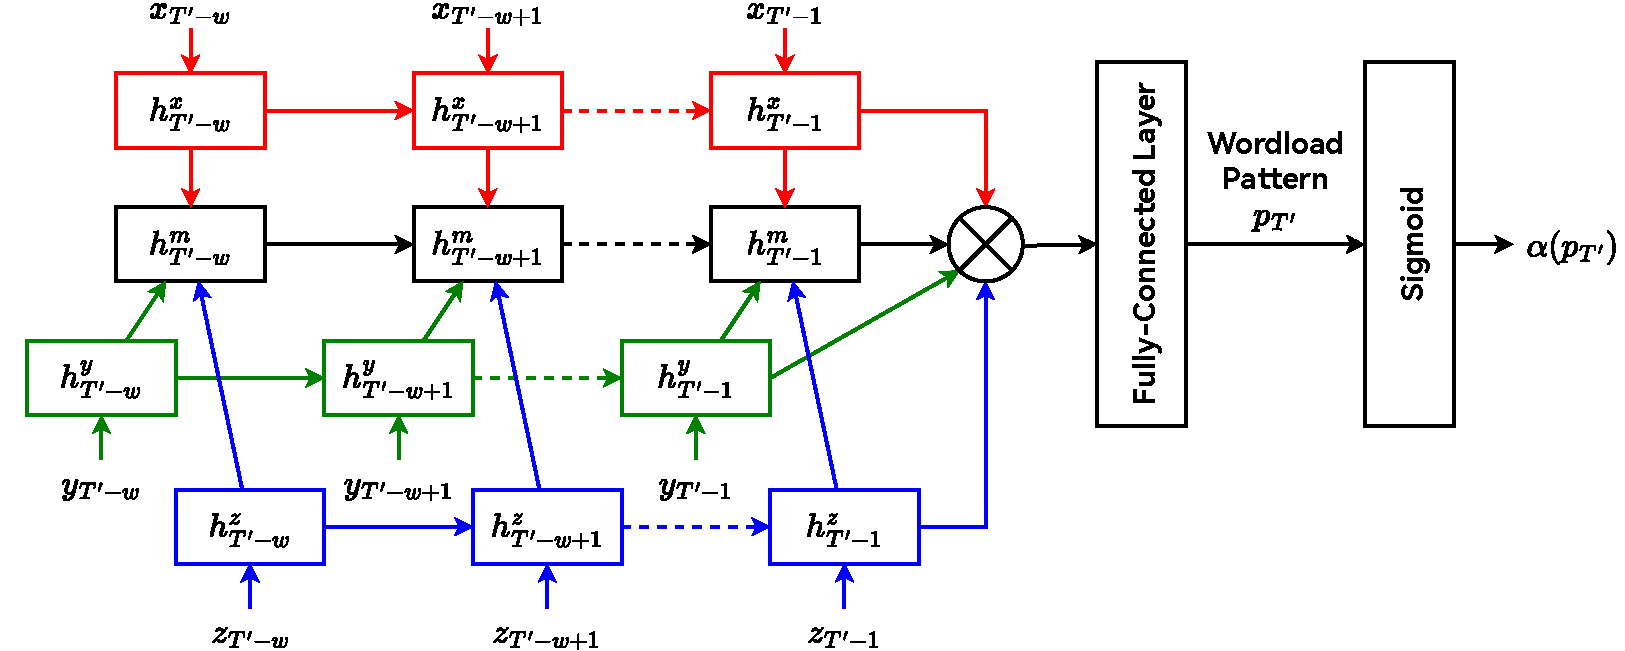
\includegraphics[height=0.55\textheight]{img/method/gru.pdf}
  \end{figure}
  除了 \textit{Workload Trend} 和 \textit{Workload Amplitude} 之外,还需要考虑 \textit{Workload Level} 。其依据 $1 \sim w$ 个弹性伸缩周期 $T^\prime$ 的工作负载数量,按照 $20\%, 40\%, 60\%, 80\%$ 四个分位点划分为五个等级。
\end{frame}

\begin{frame}{Proactive Server Elastic Scaler}{Proactive Workload Pattern Recognition}
  \begin{figure}
    \centering
    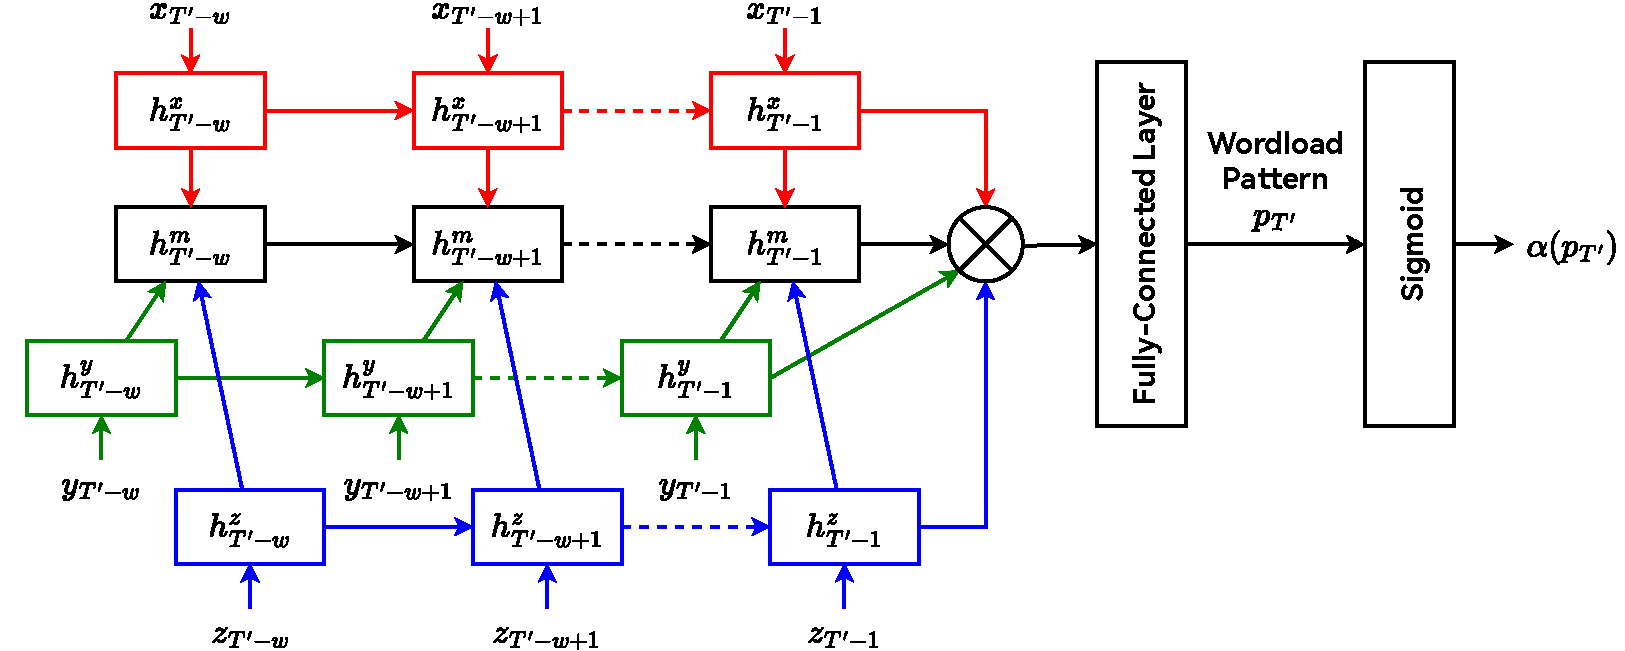
\includegraphics[height=0.55\textheight]{img/method/gru.pdf}
  \end{figure}
  \begin{equation*}
    h_{T^\prime}^x = \textcolor{red}{GRU_{level}}(x_{T^\prime}) \qquad
    h_{T^\prime}^y = \textcolor[rgb]{0,0.5,0}{GRU_{trend}}(y_{T^\prime}) \qquad
    h_{T^\prime}^z = \textcolor{blue}{GRU_{amplitude}}(z_{T^\prime})
  \end{equation*}
  $x_{T^\prime}$ ,$y_{T^\prime}$ 和 $z_{T^\prime}$ 为三种工作负载特征的历史序列;$GRU_{level}$ 、$GRU_{trend}$ 和 $GRU_{amplitude}$ 为三种特征对应的 Bi-GRU encoder ;$h_{T^\prime}^x$ 、$h_{T^\prime}^y$ 和 $h_{T^\prime}^z$ 为三种特征的隐层表示;$h_{T^\prime}^m$ 为融合特征。通过全连接层得到预测结果 $p_{T^\prime}$ ,Sigmoid 函数计算 $\alpha (p_{T^\prime})$ 用于后续服务器扩展。
\end{frame}

\begin{frame}{Proactive Server Elastic Scaler}{Server Elastic Scaling}
  根据 GRU 对工作负载模式的预测结果 $p_{T^\prime}$ ,对服务器集群进行弹性伸缩操作:
  \begin{itemize}
    \item \textit{Scaling Up}
    \item \textit{Scaling Down}
  \end{itemize}
\end{frame}

\begin{frame}{Proactive Server Elastic Scaler}{Server Elastic Scaling---Scaling Up}
  \begin{enumerate}
    \item 在弹性伸缩周期 $T^\prime$ 的\textbf{第一个}资源分配周期 $T$ 中,记录每种类型 $SC$ 的服务器的数量 $N_{T,SC}$
    \item 计算在本次弹性伸缩周期 $T^\prime$ 中,每种类型 $SC$ 的服务器需要增加的数量 $N_{T^\prime, SC}$: \[N_{T^\prime, SC} = N_{T, SC} \times \alpha (p_{T^\prime}) \times M\]
  \end{enumerate}
  \begin{itemize}
    \item $M$ 用于控制服务器新增数量的上限
    \item $\alpha (p_{T^\prime}) \in [0, 1]$ 为在不同负载模式预测结果 $p_{T^\prime}$ 下的服务器增加幅度
      \begin{align*}\alpha (S,D) &< \alpha (M,D) < \alpha (W,D) < \alpha (W,F) < \alpha (M,F) \\ &< \alpha (S,F) < \alpha (W,I) < \alpha (M,I) < \alpha (S,I)
      \end{align*} 总体而言,工作负载的波动幅度或增加趋势越大,需要增加的服务器数量越多
  \end{itemize}
\end{frame}

\begin{frame}{Proactive Server Elastic Scaler}{Server Elastic Scaling---Scaling Down}
  在服务器租期结束时,会决定是否进行缩容操作。如果服务器 $s_x$ 在到期时满足以下两个条件之一,则会被释放:
  \begin{enumerate}
    \item 在未来的资源分配周期 $T$ 内,没有函数实例计划分配到服务器 $s_x$ 上
    \item 服务器 $s_x$ 在租用期间的空闲时间或低负载时间超过一定阈值
  \end{enumerate}
\end{frame}

\begin{frame}

  \centering
  \Huge
  \usefont{OT1}{pzc}{m}{n}
  Thanks for listening!

\end{frame}

\end{document}
